\documentclass[runningheads]{llncs}
\usepackage{amssymb} 
\usepackage{booktabs}
\usepackage{graphicx}
\usepackage{microtype} % Optimizes typography to save layout space
\usepackage{cite} % Compresses multiple citations sequentially (e.g. [1,2,3] -> [1-3])
\usepackage{tikz}
\usetikzlibrary{shapes,positioning,arrows}

\begin{document}

\title{An Analytical Review of Retrieval-Augmented Generation Architectures: Addressing the Challenges of Multi-Hop Question Answering and Contextual Coherence}
\titlerunning{Analytical Review of RAG Architectures}

\author{Anonymous Authors}

\authorrunning{Anonymous}

\institute{Institution names omitted for double-blind review}

\maketitle

\begin{abstract}
Retrieval-Augmented Generation (RAG) has significantly enhanced large language models (LLMs) with external knowledge. While effective for single-hop tasks, RAG struggles with multi-hop question answering requiring complex reasoning chains. This paper introduces a problem-driven analytical framework that characterizes RAG architecture failure modes in multi-hop reasoning. We map limiting factors—including embedding bottlenecks and context fragmentation—to specific design trade-offs across Vector-based, Graph-based, and Hybrid/Agentic architectures. By explicitly evaluating these architectures against a coherence-vs-recall and retrieval-vs-reasoning lens, we derive actionable design principles and provide a unifying perspective for reasoning-aware RAG system development.
\end{abstract}

\keywords{Retrieval-Augmented Generation \and Large Language Models \and Multi-hop Question Answering \and Information Retrieval \and Reasoning}

\section{Introduction}
Retrieval-Augmented Generation (RAG) systems retrieve relevant information from external corpora during inference, addressing limitations of parametric language models such as knowledge cut-offs and hallucination \cite{1,2}. Recent work shows retrieval augmentation improves groundedness and domain adaptation across open-domain QA and long-context tasks \cite{7,23,41}.

However, RAG's limitations emerge in multi-hop question answering (QA), which requires combining multiple dependent facts in reasoning chains. Traditional RAG architectures optimize for semantic similarity rather than step-by-step reasoning, retrieving individually relevant but disconnected evidence \cite{13,67}. Graph-based RAG architectures organize information into knowledge graphs and entity-relation networks, enabling multi-hop reasoning through explicit relationship modeling \cite{19,54}.

Recent surveys examine RAG through architectural taxonomies \cite{3,4,5}, but treat multi-hop QA merely as an application-level concern. We present the first problem-driven analytical framework directly linking architectural design choices to multi-hop reasoning failure modes. By explicitly emphasizing the trade-offs between retrieval efficiency versus reasoning accuracy, and coherence versus recall, we pivot from a conventional survey approach toward establishing formal structural design principles. Table~\ref{tab:survey_comparison} presents a detailed comparison with existing surveys.

\begin{table*}[htbp]
\centering
\caption{Comparison of Feature Coverage Across RAG Survey Papers}
\label{tab:survey_comparison}
\setlength{\tabcolsep}{10pt}
\begin{tabular}{@{}lcccc@{}}
\toprule
\textbf{Key Aspects \& Coverage} & \textbf{Gao et al.} & \textbf{Ma et al.} & \textbf{Wu et al.} & \textbf{Our Work} \\
 & \cite{3} & \cite{4} & \cite{5} & \\ 
\midrule
\multicolumn{5}{l}{\textit{Architectural Scope}} \\
\quad Vector-Based RAG & $\checkmark$ & & $\checkmark$ & $\checkmark$ \\
\quad Graph-Based RAG & & $\checkmark$ & & $\checkmark$ \\
\quad Hybrid \& Agentic Architectures & $\checkmark$ & & & $\checkmark$ \\
\midrule
\multicolumn{5}{l}{\textit{Primary Problem Focus}} \\ 
\quad Multi-Hop Question Answering & & & & $\checkmark$ \\
\quad Contextual Coherence & & & & $\checkmark$ \\
\quad Fact Verification / Grounding & & & $\checkmark$ & $\checkmark$ \\
\quad KG Construction \& Quality & & $\checkmark$ & & $\checkmark$ \\
\midrule
\multicolumn{5}{l}{\textit{Analytical Depth}} \\
\quad Failure Mode Analysis & & & & $\checkmark$ \\
\quad Analysis of Embedding Bottlenecks & & & & $\checkmark$ \\ 
\quad Reasoning-Aware Retrieval & & $\checkmark$ & & $\checkmark$ \\
\bottomrule
\end{tabular}
\end{table*}

\textbf{Contributions:}
\begin{itemize}
\item Formulation of an analytical framework linking RAG architectural design to multi-hop reasoning failure modes
\item Systematic identification of architectural failure modes (embedding bottlenecks, context fragmentation, weak retrieval-reasoning integration)
\item Comparative analysis evaluating Vector-based, Graph-based, and Hybrid/Agentic models through a performance trade-off lens
\item Derivation of structural design principles for developing reasoning-aware RAG systems
\end{itemize}


\section{Problem Analysis: Limitations of RAG in Multi-Hop QA}

To formalize our analytical framework, Figure~\ref{fig:failure_modes} illustrates how standard RAG pipelines fail during complex deduction. Multi-hop QA exposes fundamental RAG limitations less visible in single-hop settings. Unlike factoid queries, multi-hop QA requires combining interdependent facts to form reasoning chains.

\begin{figure}[ht]
\centering
\resizebox{0.9\textwidth}{!}{%
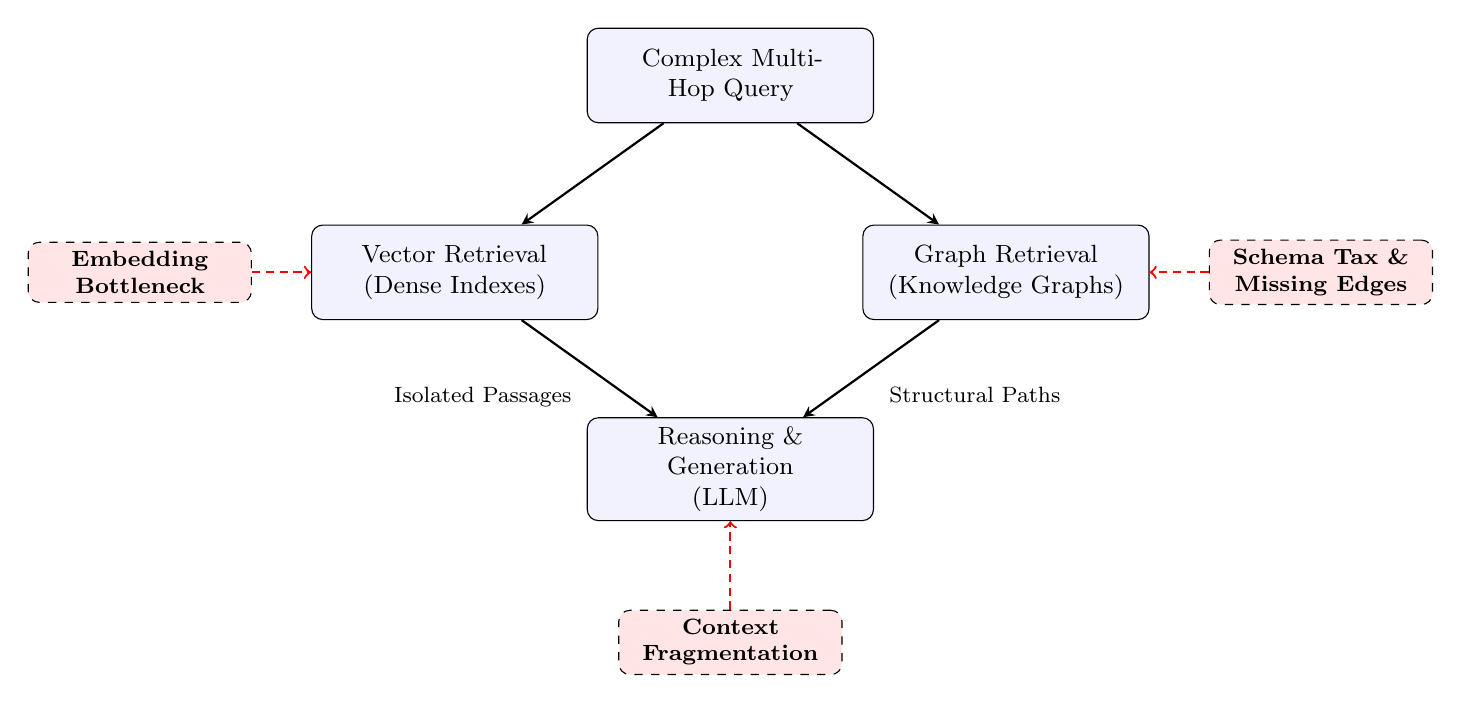
\begin{tikzpicture}[
  box/.style={rectangle, draw, rounded corners, align=center, fill=blue!5, minimum height=1.2cm, text width=3.4cm, font=\small},
  failure/.style={rectangle, draw, fill=red!10, align=center, rounded corners, dashed, text width=2.6cm, font=\footnotesize\bfseries},
  arrow/.style={->, thick, >=stealth}
]

% Main Pipeline Nodes
\node[box] (query) at (0, 0) {Complex Multi-Hop Query};
\node[box] (vector) at (-3.5, -2.5) {Vector Retrieval\\(Dense Indexes)};
\node[box] (graph) at (3.5, -2.5) {Graph Retrieval\\(Knowledge Graphs)};
\node[box] (llm) at (0, -5) {Reasoning \& Generation\\(LLM)};

% Failure Nodes
\node[failure] (embed) at (-7.5, -2.5) {Embedding\\Bottleneck};
\node[failure] (tax) at (7.5, -2.5) {Schema Tax \&\\Missing Edges};
\node[failure] (frag) at (0, -7.2) {Context\\Fragmentation};

% Main Edges
\draw[arrow] (query) -- (vector);
\draw[arrow] (query) -- (graph);
\draw[arrow] (vector) -- (llm) node[midway, below left=0.1cm and 0.1cm] {\footnotesize Isolated Passages};
\draw[arrow] (graph) -- (llm) node[midway, below right=0.1cm and 0.1cm] {\footnotesize Structural Paths};

% Failure Edges
\draw[->, red, densely dashed, thick] (embed) -- (vector);
\draw[->, red, densely dashed, thick] (tax) -- (graph);
\draw[->, red, densely dashed, thick] (frag) -- (llm);
\end{tikzpicture}%
}
\caption{Analytical framework mapping architectural dependencies to specific failure modes in RAG multi-hop reasoning.}
\label{fig:failure_modes}
\end{figure}

\subsection{Fixed-Dimensional Embedding Bottleneck}

Vector-based RAG systems compress queries and documents into fixed-dimensional embeddings for nearest-neighbor retrieval \cite{6,7}. While effective for semantic similarity, this creates limitations for compositional queries requiring specific fact combinations whose relevance cannot be determined through independent similarity scores. Research shows single-vector models fail at complex query-document relationships requiring simultaneous multi-condition matching \cite{8}. Late-interaction models like ColBERT maintain token-level representations \cite{9} but retrieve passages independently without explicit reasoning paths \cite{10}, causing dense retrievers to return semantically related but logically disconnected passages — a silent retrieval failure.

\subsection{Context Fragmentation from Chunk-Based Retrieval}

Context fragmentation occurs when semantically related content is divided into disconnected segments. Fixed-size chunking disrupts logical relationships, requiring generation systems to reconstruct missing connections. While overlapping chunks offer a marginal improvement, they still fail to preserve the broader narrative structure required for multi-hop deduction. Studies show chunk-based retrieval reduces performance on multi-step reasoning despite relevant information being available \cite{11}. Models exhibit strong biases toward specific evidence types, ignoring fragmented or improperly structured information \cite{12}.

\subsection{Knowledge Graph Construction Quality}

Graph-based RAG performance depends on automatically generated knowledge graph quality. Entity extraction, relation identification, and cross-document alignment introduce errors creating incomplete graph structures \cite{14,15}. Graph construction errors propagate through both retrieval and generation — missing edges halt reasoning paths. While structured knowledge integration benefits language models \cite{16}, ontology mismatches and alignment errors remain challenging \cite{17}.

\subsection{Limited Graph Structure Utilization}

Most graph-based RAG systems convert graph nodes to embeddings for similarity-based retrieval, treating graphs as unstructured indexes without leveraging relational connections \cite{18}. Reasoning-oriented models like QA-GNN demonstrate that preserving graph topology enables multi-hop inference through message passing \cite{19,20}. However, embedding-centric pipelines discard structural signals, functioning like standard vector retrieval \cite{21}.

\subsection{Semantic Coherence Across Hops}

Multi-hop QA requires retrieving correct facts while preserving semantic connections between evidence sources. Reasoning breaks down when handling differences in expression, temporal references, and numerical systems. Research shows maintaining coherence between reasoning steps is more important than increasing passage count \cite{22,23}. Semantic misalignment between steps creates cumulative effects leading to hallucinated connections \cite{24}.

\subsection{Cost, Benchmarking, and Integration Gaps}

Multi-hop QA requires multiple retrieval rounds, increasing computational costs as inference expenses grow with retrieval steps \cite{26}. Evaluation benchmarks compound this challenge by assessing single-hop relevance rather than compositional reasoning: while HotpotQA and MuSiQue provide multi-hop supervision \cite{28,29}, dataset artifacts enable shortcut exploitation rather than genuine multi-step reasoning \cite{30}. Most critically, RAG pipelines follow retrieve-then-generate workflows where retrieval and reasoning operate independently, preventing intermediate reasoning from guiding subsequent retrieval \cite{23,67}.


\section{Vector-Based RAG Architectures}

Vector-based RAG systems transform queries and documents into dense semantic vectors for approximate nearest-neighbor search. Dense encoders \cite{31,32} achieve substantially better retrieval than lexical methods such as BM25, enabling large-scale open-domain QA, but multi-hop reasoning capabilities remain limited.

\subsection{Dense Retrieval and the Embedding Bottleneck}

Dense Passage Retrieval (DPR) creates fixed-dimensional vectors enabling efficient nearest-neighbor search but introduces the embedding bottleneck for compositional queries \cite{7}. Extensions like REALM incorporate retrieval supervision within end-to-end QA pipelines \cite{2,35}, while ANCE and RocketQA use hard-negative mining and cross-encoder distillation \cite{36,43}. Despite improvements, models maintain independent passage scoring and return semantically related but logically irrelevant passages in multi-hop tasks, relying on shortcut correlations rather than compositional reasoning \cite{38,47}.

\subsection{Late-Interaction, Multi-Vector, and Query Transformation}

ColBERT maintains token-level embeddings calculating relevance through maximum similarity matching \cite{9}. ColBERTv2 improves speed through residual quantization \cite{39}, PLAID enables scalable real-time retrieval \cite{40}, and SPLADE combines lexical matching with semantic representations \cite{42}. Multi-vector techniques increase representational capacity but retrieved passages remain separate units without explicit reasoning paths \cite{41}. Query decomposition approaches such as HyDE \cite{89} and Step-Back Prompting \cite{90} enhance retrieval coverage but cannot expose inter-document relationships encoded in fixed vector indexes.


\section{Graph-based RAG Architectures}

Graph-based mechanisms extend retrieval by using relational knowledge triples for explicit reasoning path tracking \cite{14,48}, though automatic graph construction from unstructured text remains noisy \cite{14,15}.

\subsection{Foundations and Modern Graph Systems}

Graph neural networks (GNNs) dictate multi-step reasoning via relational inductive biases \cite{20}, a foundation established by models like GraftNet \cite{79} and EmbedKGQA \cite{81}, and extended by modern neural-symbolic traversal \cite{82,83}. Currently, systems like QA-GNN \cite{19} pass messages across entity graphs to bridge gaps. Frameworks such as GraphRAG \cite{54} and Clue-RAG \cite{57} utilize hierarchical clustering for global queries, while GNN-RAG \cite{56} and UniKGQA \cite{58} jointly optimize path discovery and reasoning.

\subsection{Limitations and Failure Modes}

Graph-based RAG faces three major challenges: scalability, expense, and adaptability. The main obstacle is the ``construction tax'' — building reliable graphs from unstructured text requires intensive computational resources. ``Schema rigidity'' creates another obstacle: predefined schemas limit use in open-domain environments where knowledge changes rapidly. Additional challenges include incomplete graphs and extraction errors obstructing traversal paths \cite{15,59}, coverage limitations in large curated graphs \cite{15,59}, and GNN reasoning struggling with compositional queries and sparse connections \cite{21}. Evaluation on benchmarks like HotpotQA, WebQuestionsSP, and ComplexWebQuestions \cite{28,61,62} shows improvement, but annotation artifacts mean benchmark gains do not always reflect genuine open-domain multi-hop reasoning capability.


\section{Hybrid and Agentic RAG Systems}

Hybrid systems extend the retrieve-then-generate paradigm. Exposing intermediate reasoning via Chain-of-Thought \cite{63} and dynamic tool actions (ReAct) \cite{64} allows agents to orchestrate retrieval natively based on evolving contexts.

\subsection{Iterative Decomposition and Tool Orchestration}

Self-Ask \cite{38} and Least-to-Most prompting \cite{66} break multi-hop queries into chronological sub-queries, drastically minimizing the retriever's search space. Inference-based models use these incomplete responses to guide subsequent retrieval \cite{67,68}, forging more coherent connections than static top-$k$ logic. Expanding this, tool-using architectures \cite{69,86,87,88} demonstrate that iterative search loops boost empirical accuracy. Think-on-Graph \cite{71} merges KG traversal with dense vectors, DSP \cite{72} executes symbolic planning, and FrugalRAG \cite{73} leverages RL-policies to slash API costs. However, vulnerabilities persist: sequential loops amplify early mistakes, and most agentic layers rely entirely on heuristic prompting rather than task-specific retrieval-reasoning training objectives.


\section{Comparative Analysis}

Table~\ref{tab:comparison} shows vector-based retrievers prioritize efficiency while graph and agentic RAG deliver better multi-hop reasoning at increased preprocessing and inference costs.

\subsection{Evaluation Axes and Metrics}

\textbf{Multi-Hop Reasoning Accuracy} is assessed using Exact Match (EM) and F1 metrics on HotpotQA \cite{28}, WebQuestionsSP \cite{61}, 2WikiMultiHopQA \cite{75}, and MuSiQue \cite{29}. \textbf{Contextual Coherence} evaluates whether retrieved evidence establishes logical frameworks supporting deductive reasoning \cite{11,12}.

\subsubsection{RAG-Specific Faithfulness Frameworks}
The evaluation frameworks \textbf{RAGAS (Retrieval Augmented Generation Assessment)} \cite{91} and \textbf{ARES} \cite{92} have been developed to decrease hallucination problems that affect retrieval-augmented systems. These frameworks break down results into multiple detailed metrics which assess different elements of the retrieval-to-generation workflow:
\begin{itemize}
\item \textbf{Context Precision/Recall:} Assesses relevance of retrieved passages and whether they sufficiently cover required information.
\item \textbf{Faithfulness:} Evaluates if the output is strictly supported by retrieved evidence without hallucinated knowledge.
\item \textbf{Answer Relevance:} Measures how directly the generated output addresses the user's intent.
\end{itemize}
The combination of these metrics provides a complete assessment method for locating where the retrieval-to-generation pipeline fails.

\subsubsection{LLM-Based Evaluation (LLM-as-a-Judge)}
Traditional lexical metrics like EM and F1 penalize correct answers formulated with different terminology. To address this, evaluations increasingly utilize LLM-as-a-Judge frameworks \cite{93}, where advanced language models structured with specific prompts assess generated responses based on meaning, factual grounding, and overall quality. This effectively establishes valid reasoning as correct despite surface-level text variations.

\vspace{1em}
\noindent \textbf{Retrieval Efficiency} covers query latency, throughput, and token consumption — ColBERT achieves 170$\times$ lower latency than cross-encoder reranking \cite{9}, and FrugalRAG halves retrieval costs \cite{73}. \textbf{Retrieval-Reasoning Integration} evaluates end-to-end performance from simultaneous optimization \cite{58,72}.

Table~\ref{tab:comparison} presents a structured comparison of the surveyed systems against these metrics. We focus on HotpotQA results where available, as it serves as the primary benchmark for multi-hop reasoning.

\begin{table}[ht]
\caption{Comparative Analysis of RAG Architectures}
\label{tab:comparison}
\centering
\resizebox{\textwidth}{!}{%
\begin{tabular}{p{2cm} p{1.5cm} p{3.5cm} p{3.5cm} p{3.5cm} p{2cm} p{2cm}}
\toprule
\textbf{System} & \textbf{Category} & \textbf{Key Mechanism} & \textbf{Strengths} & \textbf{Limitations} & \textbf{HotpotQA (F1/EM)} & \textbf{Latency/ Calls} \\
\midrule
\textbf{ColBERT} \cite{9} & Vector & BERT-based multi-vector late-interaction & Competitive retrieval (MRR@10 $\approx$36.7); 170$\times$ faster than BERT re-ranking & No multi-hop support; Very large index & N/A & $\sim$5--6 ms (1 call) \\
\midrule
\textbf{DPR} \cite{7} & Vector & Dense bi-encoder (Question / Passage) & High passage recall (78.4\% on NQ); Sample efficient & No explicit multi-hop reasoning; Embedding bottleneck & N/A & $\approx$10 ms (1 call) \\
\midrule
\textbf{KG\textsuperscript{2}RAG} \cite{76} & Hybrid/ Graph & KG-guided chunk expansion \& organization & Improves multi-hop QA (HotpotQA F1 66.3); Robust to KG noise & Requires KG index; Dependent on KG quality & 66.3 (F1) & 1 call \\
\midrule
\textbf{GNN-RAG} \cite{56} & Graph & GNN-based node weighting \& path retrieval & Strong KG-QA performance; +8.9--15.5\% F1 on multi-hop & Only for structured KGQA; No open-text eval & N/A & 1 call \\
\midrule
\textbf{Clue-RAG} \cite{57} & Graph & Multi-partite graph + iterative retrieval & Dramatic QA gains (+113.5\% F1 over SOTA); Low indexing cost & Complex index; Heavy preprocessing & N/A & 1 call \\
\midrule
\textbf{HiRAG} \cite{77} & Graph/ Hierarchical & Hierarchical KG indexing \& retrieval & High multi-hop QA accuracy; Compact prompts & Expensive offline indexing; Precompute overhead & 73.7 (F1) / 65.5 (EM) & 1 call \\
\midrule
\textbf{SCMRAG} \cite{78} & Hybrid & Self-corrective agent + dynamic KG augmentation & Improves retrieval-heavy QA (67.6\% vs 56.0\%); Dynamic updates & Complex agentic pipeline; Relies on web search & 67.6 (Acc) & Multi-step \\
\midrule
\textbf{SimGRAG} \cite{55} & Graph & Semantic subgraph retrieval (KG search) & Near-perfect KGQA retrieval (Hits@1 $\approx$98\%); Precise subgraphs & Only for KGQA (no text corpus); Computationally expensive & N/A & 1 call \\
\midrule
\textbf{FrugalRAG} \cite{73} & Hybrid & RL-based adaptive retrieval-step reduction & Maintains accuracy while halving retrieval cost (tokens) & Requires RL fine-tuning; Complexity & N/A & 1 call \\
\midrule
\textbf{DSP} \cite{72} & Pipeline & Demonstrate-Search-Predict orchestration & Significant gains on open-domain QA (8--39\% relative) & Manually designed prompts; Not end-to-end trainable & N/A & Multi-step \\
\bottomrule
\end{tabular}%
}
\end{table}

Table~\ref{tab:comparison} demonstrates vector-based systems (DPR, ColBERT) maintain query processing under 10ms but lack multi-hop reasoning capabilities. Graph-based and hybrid systems (KG2RAG, HiRAG, SCMRAG) achieve much better HotpotQA results, with HiRAG reaching F1 scores of \textbf{73.7}. However, performance improvements require more complex designs and additional data processing. SCMRAG and DSP demonstrate movement toward agent-based computation with dynamic retrieval choices but require multiple model invocations increasing inference times.

The comparison reveals competing interests requiring balance. Vector-based systems focus on fast retrieval and scalability, while graph-based systems deliver structured reasoning and contextual understanding. Current systems fail to achieve optimal performance across speed, reliability, and multi-hop reasoning, indicating future systems need better retrieval-inference integration.


\section{Discussion and Future Directions}

RAG has achieved major progress yet design limitations restrict multi-hop QA capabilities. Fixed-capacity embeddings prevent necessary content connections while fragmented contextual inputs break reasoning processes.

\subsection{Silent Failures, Fragmentation, and the Construction Tax}

Standard dense retrieval creates silent failures: retrievers identify isolated relevant sections even when queries require combined essential evidence, presenting seemingly reliable but incomplete context \cite{9,10}. Fixed-size chunking compounds this by breaking logical relationships between connected sections \cite{11}. Graph-based methods display similar restrictions when incomplete reasoning paths obstruct connection generation. ``Semantic unit'' processing — dividing documents by logical components rather than token thresholds — offers a path forward: Meta-Chunking \cite{11} and Landmark Embeddings \cite{12} use LLMs to identify semantically meaningful boundaries while maintaining sentence-level relationships. Graph-based RAG faces an additional ``construction tax'': entity extraction, relation identification, and schema alignment require substantial resources, and many graph RAG systems ultimately degrade to vector similarity search without utilizing topological structure \cite{15,21}.

\subsection{Paradigm Convergence and Reasoning-Aware Agents}

Traditional distinctions between vector and graph-based retrieval will diminish. Future systems will unify semantic similarity search and structured graph traversal through multi-vector representations approximating graph topology — MUVERA \cite{10} demonstrates fixed-dimensional encodings that approximate multi-vector Chamfer similarity at DPR-like speeds, enabling implicit graph-like connectivity without symbolic edges. Simultaneously, the retrieve-then-generate paradigm must give way to reasoning-aware retrieval: RaDeR \cite{68} uses chain-of-thought supervision with hard negatives from failed reasoning attempts, and SCM-RAG \cite{78} builds knowledge graphs dynamically while refining queries through new evidence, treating retrieval as a continuous process interleaved with reasoning \cite{67}.

Furthermore, hybrid tool-using architectures \cite{69,87,88} are proving essential for navigating complex query landscapes. By exposing reasoning APIs and database engines as callable capabilities, language models can independently orchestrate fact retrieval from disparate databases, shifting the structural burden away from static indexes and toward dynamic execution environments. However, scaling these agentic workflows to production environments will necessitate more robust error correction and rollback mechanisms to prevent early hallucination cascades from permanently corrupting down-stream inference chains.

\subsection{Holistic Evaluation}

Future evaluation frameworks must assess reasoning processes beyond answer correctness, penalizing correct answers derived from flawed reasoning chains while rewarding evidence-grounded inference patterns. Methodologies should explicitly incorporate adversarial perturbation of source documents to test whether RAG models can dynamically adjust their reasoning paths or if they rigidly depend on shortcut correlations. This enables assessment of both operational accuracy and transparent, interpretable decision-making.


\section{Conclusion}

This paper establishes a formal analytical framework linking RAG architectural designs directly to their failure modes in multi-hop reasoning. We demonstrate that while vector-based retrieval scales efficiently, its fixed-dimensional embeddings fundamentally bottleneck compositional reasoning. Graph-based RAG provides explicit structural reasoning pathways but imposes a severe schema construction tax and noise susceptibility. Hybrid and agentic designs bridge the retrieval-reasoning gap through dynamic orchestration, though at significant architectural cost. By formalizing these structural trade-offs—specifically coherence versus recall and retrieval efficiency versus reasoning accuracy—we conclude that overcoming context fragmentation and embedding constraints requires abandoning static retrieve-then-generate pipelines. Future reasoning-aware systems must jointly optimize retrieval and inference as an interleaved, dynamically evaluated process to achieve genuinely robust multi-hop deduction.

\bibliographystyle{splncs04}
\bibliography{references}

\end{document}